Interactions between matter particles are mediated by spin=1 particles called gauge bosons. These particles are required to preserve the local gauge symmetry of the Standard Model Lagrangian. \footnote{A Lagrangian is said to possess a local gauge symmetry if it is invariant under a particle wave function rotation that is dependent on the space-time position of the particle.} An example of this principle is the electromagnetic interaction which is a U(1) gauge theory. In this theory, the charged particle wave-function is transformed as shown in Eq.~\ref{charged}.

\begin{equation} 
\label{charged}
|\Psi>^{'} = e^{iq\theta(x)}|\Psi>
\end{equation}

The requirement that the electromagnetic Lagragian remain invariant under this transformation requires the existence of a photon field that couples to all charged particles. The amount to which this new field couples to charged particles is given by the value of $q$ (i.e. the electric charge of the particle).

  such as a rotation shown in Eq.~\ref{gauge}.

\begin{equation}
\label{gauge}
|\Psi>^{'} = e^{i\vec{\alpha} \bullet \vec{\theta}(x)}|\Psi>
\end{equation}

where $\vec{\alpha}$ and $\vec{\theta}$(x) are N-dimensional vectors and N represents the size of the rotation group. Because the Standard Model Lagrangian includes space-time derivatives of the wave-function, additional terms will appear which correspond to a new field that couples to the matter particle. These new fields are required to preserve the symmetry group structure of the Lagrangian and result in an interaction term which couples the matter fields with the newly formed gauge field.

\subsection{Electroweak Unification and Symmetry Breaking}
\label{electroweak}

One of the crowning achievements of theoretical physics in the twentieth century is the unification of the electromagnetic and weak interactions. The electromagnetic interaction occurs between particles with electric charge, such as an electron with charge $\pm1$ or a up quark with charge $\pm\frac{2}{3}$. The weak interaction, at low energies, is seen almost solely in nuclear beta decay such as neutron decay or muon decay. The weak interaction is named so because the strength of the interaction is much lower than the electromagnetic or strong interactions. The unification of these two forces is described by the combined symmetry group \mbox{SU(2)$_{L}$ $\otimes$ U(1)$_{Y}$}, where the subscript L refers to the property of the weak interaction that is only couples to left-handed particles and right-handed anti-particles\footnote{A particle is defined as left-handed if its spin is anti-aligned with its momentum ($\hat{s}\bullet\hat{p}=-1$). A right-handed particle has its spin aligned with its momentum vector ($\hat{s}\bullet\hat{p}=1$).}, and the subscript Y is called weak hypercharge which is related to the electric charge. The unification of these two interactions is remarkable because it correctly predicts the presence of two charged bosons (W$^{\pm}$) and two neutral bosons (B and W$^{0}$). The charged bosons are needed to explain charged current interactions such as muon decay ($\mu^{-}\rightarrow e^{-} \bar{\nu}_{e} \nu_{\mu}$) and the neutral bosons are required to explain the existence of neutral current interactions ( $e^{+}e^{-} \rightarrow \mu^{+}\mu^{-}$).

While the unification of the electromagnetic and weak interactions is remarkable it has one major problem: The W$^{\pm}$ and Z boson are, by contruction, required to have zero mass which highly inconsistent with their measured masses of 80.4 and 91.2 GeV, respectively. The non-zero masses imply that the underlying \mbox{SU(2)$_{L}$ $\otimes$ U(1)$_{Y}$} group is not a true symmetry of nature and is said to be a ``broken" symmetry. One way to break the symmetry is to add a term, which is a function of a new scalar field, $\phi=\left( \phi_{1}~\phi_{2} \right)^{T}$, to the electroweak Lagrangian. This new term in the Lagrangian, shown in Eq.~\ref{Higgs}, has the canonical kinetic term ($\partial\phi^{\dagger}\partial\phi$) and a potential term ($V(\phi)=\mu^{2}\phi^{\dagger}\phi + h(\phi^{\dagger}\phi)^{2}$) that has a ``wine bottle" shape shown in Fig.~\ref{HiggsPotential}.

\begin{equation}
\label{Higgs}
\mathcal{L} = \partial\phi^{\dagger}\partial\phi - \mu^{2}\phi^{\dagger}\phi - h(\phi^{\dagger}\phi)^{2}
\end{equation}

\begin{figure}[!h!tbp]
\begin{center}
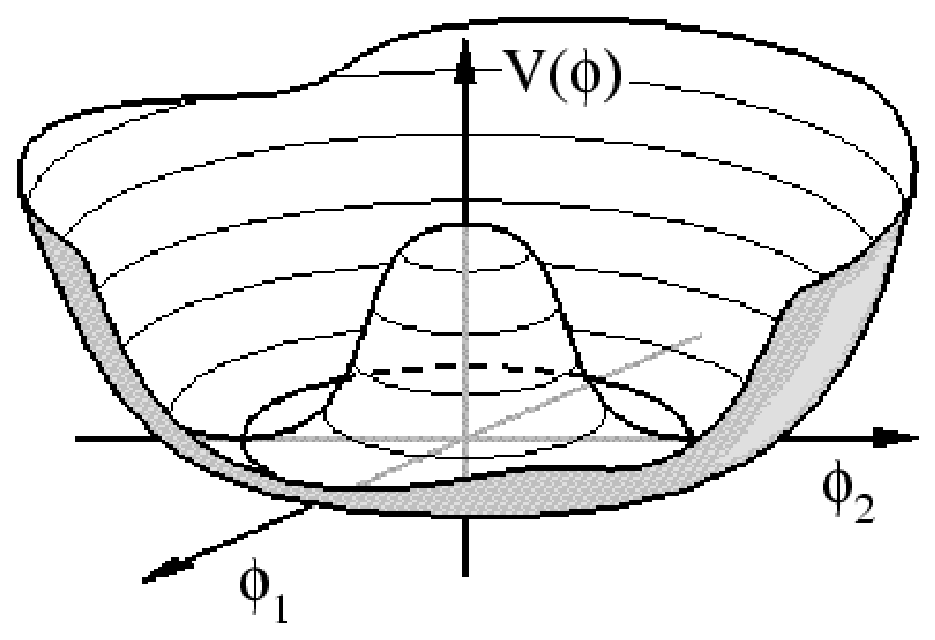
\includegraphics[width=0.75\textwidth]{eps/Theory/HiggsPotential.eps}
\end{center}
\vspace{-0.1in}
\caption{The Higgs "wine-bottle" potential.}
\label{HiggsPotential}
\end{figure}

The result of adding this new term in the electroweak Lagrangian is for the vacuum ground state to acquire an expectation value (VEV) defined by the minimum of this potential shown in Fig.~\ref{HiggsPotential}. The result of the new vacuum expectation value is to break the \mbox{SU(2)$_{L}$ $\otimes$ U(1)$_{Y}$} symmetry of the electroweak Lagrangian and allow the $W$ and $Z$ to acquire mass while the photon remains massless. This method of breaking electroweak symmetry is known as the Higgs mechanism and predicts the existence of one massive scalar (i.e. spin=0) boson known as the Higgs boson. The existence of the Higgs boson has not been experimentally verified and it's discovery remains one of the outstanding challenges in experimental high energy physicists.


\subsection{Strong Interactions}
\label{strong}

The strong interaction is the force which binds the proton together and is named so because the relative coupling strength is much larger than the electromagnetic or weak interaction. The strong interaction is mediated by eight massless gluons which result from the invariance of the strong Lagrangian under a local SU(3) rotation of the quark fields. The eight gluons allow interactions between any particle that carries a color charge\footnote{The color charge is similar to the electric charge except there are three color charges compared to one electric charge. The three colors are commonly called red (R), blue (B), and green (G).}. Quarks and gluons themselves are the only fundamental particles that carry color charge. An interesting property of the strong interaction is color confinement, which states that at low energies a bare quarks can not travel long distances when they carry color charge. Instead, colored quarks combine with other quarks to form colorless bound states called mesons or baryons depending on the number of constituent quarks. The process of forming bound states is called hadronization. The top quark, discussed in the section~\ref{topquark}, is the only quark that does not undergo hadronization due its extremely short lifetime.
The strong interaction exhibits an interesting property that the strength of the interaction decreases as the energy of the processes increases. Eq.~\ref{alphas}~shows the strong coupling parameter, $\alpha_{S}$, dependence on the energy of the process. 

\begin{equation}
\label{alphas}
\alpha_{S}(E) = \frac{12\pi}{33-2n_{f}\ln\left[\left(\frac{E}{\Lambda}\right)^{2}\right]}
\end{equation}

\noindent $n_{f}$ is the number of active\footnote{The number of active quark flavors depends on the energy of the process. At energies of $\sim100$ MeV, there are three quark flavors (u,d,s). At higher energies of $\sim10$ GeV, there are five quark flavors (u,d,s,c,b).} quark flavors and $\Lambda$ is the natural scale at which the strong interaction becomes ``weak" ( $\Lambda~\sim~$200 MeV).
The decreased coupling strength at energies greater than $\Lambda$ allows quarks to break their confined states and travel as bare color charges. As the quark begins to propagate however, it polarizes the vacuum between itself and its color partner until it becomes energetically favorable to create a new quark-antiquark pair. This process can repeat itself many times with a net effect of creating of a large number of strongly interacting particles traveling in the same direction as the originating colored particle. 


